\documentclass[../main.tex]{subfiles}
\begin{document}

\chapter{Transcriptome-wide association study of schizophrenia and 
chromatin activity yields mechanistic disease insights}
\labch{gusev2018}

\begin{external_abstract}{title=Abstract}
Genome-wide association studies (GWAS) have identified over 100 risk 
loci for schizophrenia, but the causal mechanisms remain largely 
unknown. We performed a transcriptome-wide association study (TWAS) 
integrating a schizophrenia GWAS of 79,845 individuals from the 
Psychiatric Genomics Consortium with expression data from brain, blood, 
and adipose tissues across 3,693 primarily control individuals. We 
identified 157 TWAS-significant genes, of which 35 did not overlap a 
known GWAS locus. Of these 157 genes, 42 were associated with specific 
chromatin features measured in independent samples, thus highlighting 
potential regulatory targets for follow-up. Suppression of one 
identified susceptibility gene, mapk3, in zebrafish showed a significant 
effect on neurodevelopmental phenotypes. Expression and splicing from 
the brain captured most of the TWAS effect across all genes. This 
large-scale connection of associations to target genes, tissues, and 
regulatory features is an essential step in moving toward a mechanistic 
understanding of GWAS.
\end{external_abstract}

\section{Introduction}

GWAS hits are difficult to explain from a mechanistical point of view, 
for the association with the disease can arise in many different 
circumstances. First of all, in the majority of cases, the GWAS hit is 
not even the real causal variant, but is merely in linkage 
disequilibrium with it; even if we knew which is the actual causal 
variant, however, we still could not infer much about its functional 
role without a deeper knowledge of the locus where the variant lies. 
Integrating GWAS signals with a functional annotation of the genome can 
give insight into the biological mechanisms through which the variant 
affects the phenotype; in particular, it has been shown that 
schizophrenia GWAS hist were enriched in regulatory elements.

The regulatory role of a genetic region is mainly determined by its 
chromatinic state, \ie by which proteins bind that region, and its 
chromatinic state is in turn influenced either in \cis, by the altered 
DNA sequence that binds the proteins, or in \trans, by altered proteins 
which do not regulate well the locus (\ie there is a mutation in a 
protein so that it does not bind the sequence at that locus any more, or 
it works more poorly). Ultimately, however, the chromatinic state of a 
region is under genetic control, therefore we have two effects that can 
spring from a genetic variant: the association with the disease or the 
association with the chromatinic state of a region. Such effects may be 
independent or not.

by fmarotta: A variant can have two main roles: a regulatory one and/or 
a structural one. If a variant affects a TF, it can indirectly be 
associated with many genes, and potentially many diseases. Different 
variants can affect the same genes, so the same disease can be due to 
many variants, thus increasing the difficulty in finding associations: 
think about how many variants can in principle affect the expression of 
a gene! Regulatory role: it alters a binding site. Structural role: ??

The authors, exploiting the method they had previously developed, 
performed a schizophrenia TWAS relying on summary-level data from a 
published GWAS, and subsequently performed a \enquote{chromatin} TWAS in 
order to find genes whose expression was associated with a chromatin 
phenotype.\todo{approfondimento section: extended phenotype. One can 
associate so many things to a disease status: perhaps underlying each of 
them is the geneome, but looking at the genome is not powerful enough: 
let us imagine a pyramid: at the bottom there is the genome, but the 
genetic variants are so many! besides, they can alter many genes, but 
the genes are less than the variants (however, if we consider gene 
expression, it is a continuous variable so there are infinite genes... 
nay, let us settle it like this: there are 20,000 genes and theri 
variation is nearly infinite). the genes in turn alters how proteins are 
made (structurally and quantitatively), but there are less proteins than 
genes (or are there?). Proteins affects metabolism, and so on. In the 
middle there is chromatin state. sorry for the stream of consciousness.} 
They then compared the two sets of genes aiming to gain insight into the 
biological function of the genes associated with schizophrenia. Their 
approach is summarised in \reffig{gusev2018/1}.

\begin{figure}
	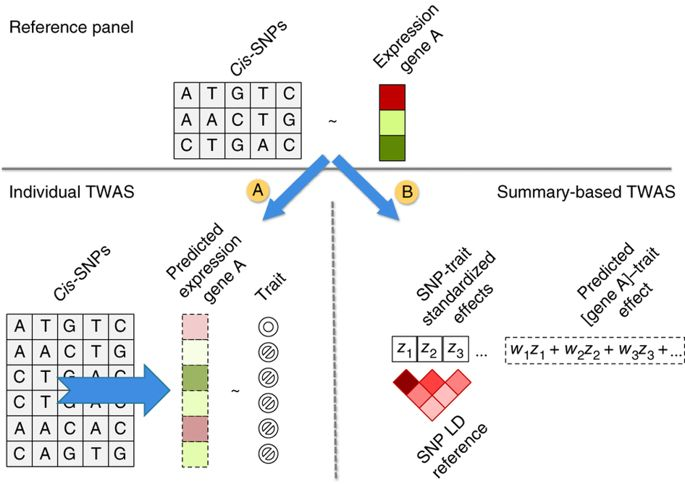
\includegraphics{gusev2018/1-TWAS_schematic}
	\labfig{gusev2018/1}
	\caption{The schematic of the TWAS approach used in the 
schizophrenia work}
\end{figure}

\section{Traning}

In this study, four datasets of either RNA-seq or genome-wide SNP-array 
expression measurements, for a total of nearly 4,000 individuals,  were 
used to train the expression models: \enquote{RNA-seq from the 
dorsolateral prefrontal cortex of 621 individuals (including 283 
schizophrenia cases, 47 bipolar cases, and 291 controls) collected by 
the CommonMind Consortium (CMC)25, expression array data measured in 
peripheral blood from 1,245 unrelated control individuals from the 
Netherlands Twin Registry (NTR)26, expression array data measured in 
blood from 1,264 control individuals from the Young Finns Study (YFS)23, 
and RNA-seq data measured in adipose tissue from 563 control individuals 
from the Metabolic Syndrome in Men study (METSIM)} (YFS/METSIM were 
pre-computed by Gamazon \etal 2015). This was not strictly necessary, 
for they could have used pre-computed weights from other works, but 
perhaps they wanted to train their models on nervous tissues expression 
data.

As previously, \cis- and \trans- heritability of gene expression were 
computed and found significant for 18,084 genes (10,819 unique). In 
addition, splicing events were characterised, since an alteration of 
this kind of regulation is implied in disease 
(http://science.sciencemag.org/content/352/6285/600).\todo{approfondire? 
I twas basano tutto sull'espressione, ma non e` l'unica cosa...}

A separate TWAS was performed for each of the four reference gene 
expression training datasets. From such datasets, a sparse midex linear 
model was used to find the weights of each \cis-SNP for each gene; also, 
linkage disequilibrium was computed from the same datasets.

\section{Schizophrenia TWAS}

247 significant genes, of which 157 unique and 35/157 completely novel, 
	were found significantly associated to the disease 
(\reffig{gusev2018/2}). Interestingly, 33 loci were found to harbour 
hotspots of multiple TWAS hits, but, after a statistical test, in 27 of 
these cases the genes were correlated, suggesting a single underlying 
effect. For instance, this could be due to an entire chromatin region 
altered, or a TF altered.

\begin{figure}
	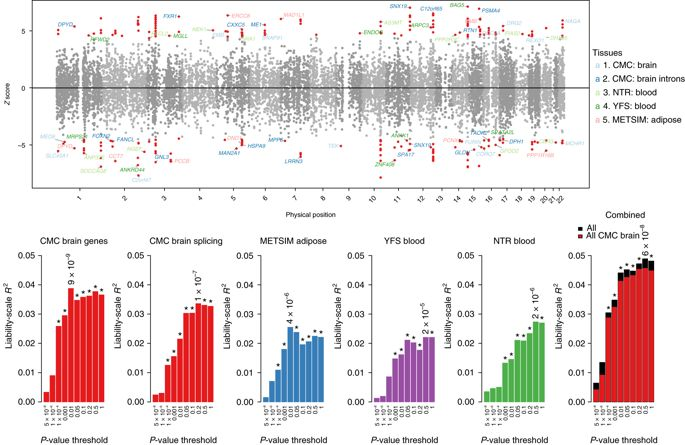
\includegraphics{gusev2018/2-schizophrenia_TWAS}
	\caption{Results of the schizophrenia TWAS}
	\labfig{gusev2018/2}
\end{figure}

Evidence emerged that TWAS are more powerful than GWAS at detecting 
multiple variants whose combined effects explain the phenotype, rather 
than events where a single variant is involved: indeed, 27\% of the 
novel genes were associated to the disease more strongly than the top 
GWAS hit at the locus of the gene, whereas only 3\% of the genes 
overlapping a reported GWAS hit were more strongly associated than the 
GWAS hit.\todo{recapitulate in the discussion}\todo{marginfigure 
supplementary 6}

46 splicing events in the brain were also found associated to the 
   disease.

skipping part on COLOC because I do not understand it.

\section{NOT Chromatin TWAS}

"A research team published a dataset of chromatin interactions, obtained 
with the Hi-C technique, in the developing human brain". The authors 
integrated the fine-mapped schizophrenia GWAS hits with the chromatin 
interaction mapping and reported 474 genes whose transcription start 
site (TSS) contacted a GWAS hit, implying that the gene's regulation was 
affected by the variant during brain development. 105 of the 157 TWAS 
significant genes were also found in this set, establishing a 
relationship between gene expression and transcriptional regulation.

skipping GE-PRS: I have to understand polygenic risk score.

\section{Chromatin TWAS}

The authors, following the lead of a previous work (refs. 6 and 18) 
collected nine chromatin markers (H3K27ac, \etc) from LCL cell lines of 
some individuals from hapmap, and treated the peaks of ChIP-seq reads as 
quantitative traits. This is an interesting example of the fact that 
phenotypes can be seen at an arbitrary level. They confirmed that gene 
expression correlated with chromatin state (see supp. fig 15).

Starting from these samples for which the chromatin phenotype was 
available, the authors imputed gene expression and splicing, then tested 
for associations between expression or splicing and chromatin state. 
Overall, an association between expression and phenotype was found for 
806 unique genes, but only 224 splicing events were associated with a 
	phenotype. \enquote{Half of the chromatin associations were 
distal... etc. see fig 24-25 supplementary}

\begin{figure}
	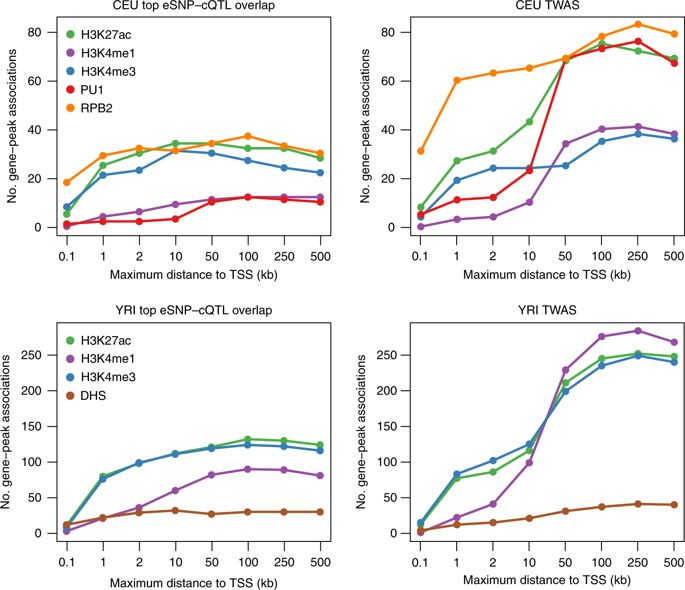
\includegraphics{gusev2018/3-chromatin_TWAS}
	\caption{Chromatin TWAS}
	\labfig{gusev2018/3}
\end{figure}

\section{Functional analysis}



\end{document}
